\chapter{Introduction}

\section{How is this book written?}

%\label{\detokenize{overview/introduction/main:introduction}}\label{\detokenize{overview/introduction/main::doc}}
This book aims to introduce readers to programming for mathematics.

It is assumed that readers are used to solving secondary school mathematics problems
of the form:


Given the function \(f:\mathbb{R}\to\mathbb{R}\) defined by
\(f(x) = x ^ 2 - 3 x + 1\) obtain the global minima of the function.


To solve this you need to apply \textbf{mathematical knowledge}:

\begin{enumerate}
    \item Differentiate \(f(x)\) to get \(\frac{df}{dx}\);
    \item Equate \(\frac{df}{dx}=0\);
    \item Use the second derivative test on the solution to the previous equation.
\end{enumerate}

For each of those 3 steps you will usually make use of our \textbf{mathematical
techniques}:
\begin{enumerate}
\item Differentiate \(f(x)\):

\begin{equation*}
\begin{split}\frac{df}{dx} = 2 x - 3\end{split}
\end{equation*}
\item Equate \(\frac{df}{dx}=0\):
\begin{equation*}
\begin{split}2x-3 =0 \Rightarrow x = 3/2\end{split}
\end{equation*}
\item Use the second derivative test on the solution:
\begin{equation*}
\begin{split}\frac{d^2f}{dx^2} = 2 > 0\text{ for all values of }x\end{split}
\end{equation*}
Thus \(x=3/2\) is the global minima of the function.

\end{enumerate}

As you progress as a mathematician \textbf{mathematical knowledge} is more prominent
than \textbf{mathematical technique}: often knowing what to do is the real problem as
opposed to having the technical ability to do it.

This is what this book will cover: \textbf{programming} allows you to instruct a
computer to carry out mathematical techniques.

For example you will learn how to solve the above problem by instructing a
computer which \textbf{mathematical technique} to carry out.

\textbf{This book covers how to give the correct instructions to a
computer.}

The following is an example, do not worry too much about the specific code used
for now:


\textbf{Differentiate \(f(x)\) to get \(\frac{df}{dx}\)}

\begin{pyin}
import sympy as sym

x = sym.Symbol("x")
sym.diff(x ** 2 - 3 * x + 1, x)
\end{pyin}

\[
    2x - 3
\]

\textbf{Equate \(\frac{df}{dx}=0\)}

\begin{pyin}
sym.solveset(2 * x - 3, x)
\end{pyin}

\[
\left\{\frac{3}{2}\right\}
\]

\textbf{Use the second derivative test on the solution}
%\label{\detokenize{overview/introduction/main:use-the-second-derivative-test-on-the-solution}}

\begin{pyin}
sym.diff(x ** 2 - 3 * x + 1, x, 2)
\end{pyin}

\[2\]

Figure~\ref{fig:knowledge_vs_technique} shows a summary.

\begin{figure}[htbp!]
\centering

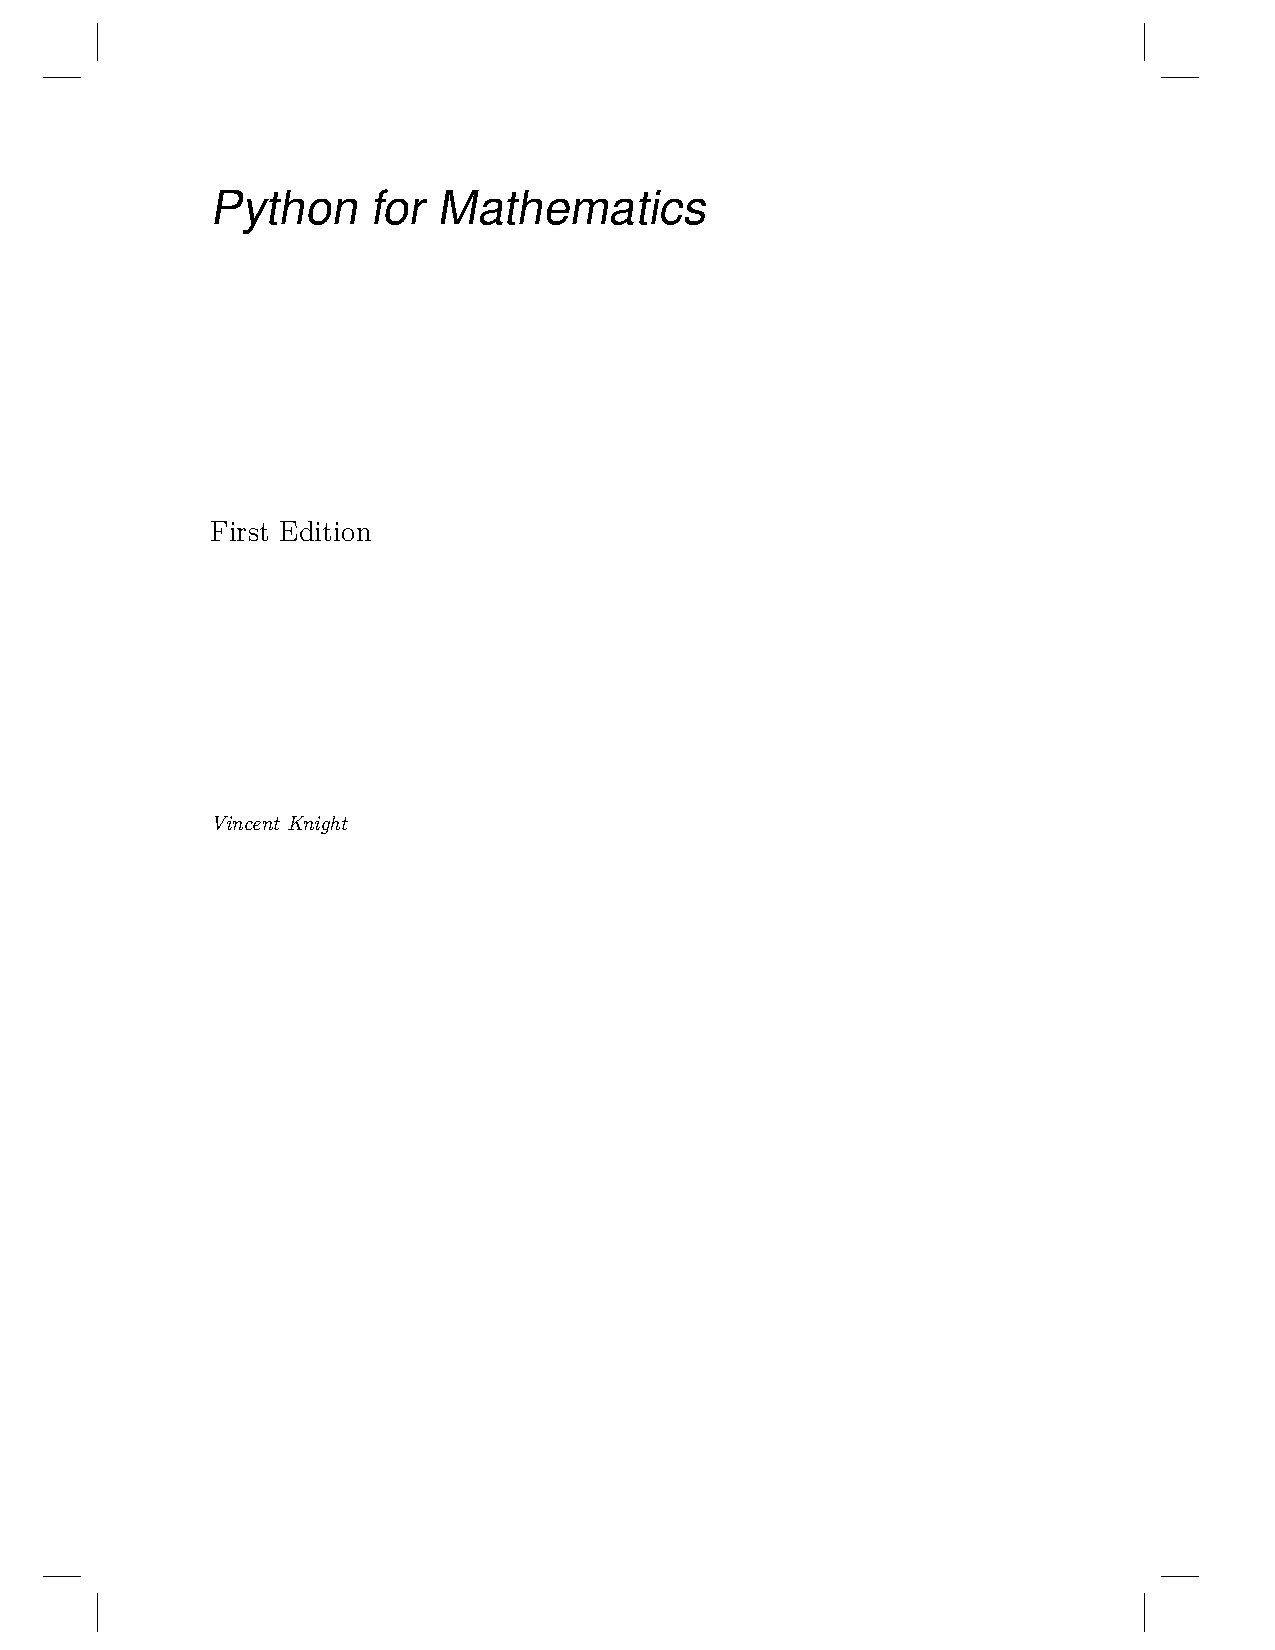
\includegraphics[width=0.75\textwidth]{assets/knowledge_vs_technique/main.pdf}
\caption{Knowledge versus technique in this
    book.}\label{fig:knowledge_vs_technique}
\end{figure}

\subsection{How is this book different from similar books?}

A traditional structure of this book would probably be to re-order the chapters
as follows:

\begin{enumerate}
    \item Chapter~\ref{chp:using_notebooks}
    \item Chapter on variables (Seen in Chapter~\ref{chp:variables_conditionals_and_loops})
    \item Chapter on conditionals (Seen in Chapter~\ref{chp:variables_conditionals_and_loops})
    \item Chapter on loops (Seen in Chapter~\ref{chp:variables_conditionals_and_loops})
    \item Chapter on functions (Seen in Chapter~\ref{chp:functions_and_data_structures})
    \item Chapters on data structures (Seen in Chapter~\ref{chp:functions_and_data_structures})
    \item Chapter~\ref{chp:objects}
    \item Chapter on Sympy (with an overview of the topics in Chapters~\ref{chp:algebra}-~\ref{chp:matrices} and~\ref{chp:differential_equations})
    \item Chapter~\ref{chp:combinatorics}
    \item Chapter~\ref{chp:probability}
    \item Chapter~\ref{chp:sequences}
    \item Chapter~\ref{chp:statistics}
    \item Chapter~\ref{chp:cli}
    \item Chapter~\ref{chp:modularisation}
    \item Chapter~\ref{chp:documentation}
    \item Chapter~\ref{chp:testing}
\end{enumerate}

The choice to \textit{flip} this structure and start with real use cases (and
not code recipes) is deliberate. The tools covered in
chapters~\ref{chp:algebra}-\ref{chp:differential_equations} can be used with
little to no programming knowledge and need only an understanding of the
mathematics. Following this, the topics
covered~\ref{chp:variables_conditionals_and_loops}-\ref{chp:objects} let the reader
expand on the knowledge and learn basics of programming. The topics and techniques covered in
chapters~\ref{chp:cli}-\ref{chp:testing} show how modern research
software is designed.

\section{What is in this book?}

%\label{\detokenize{overview/structure/main:how-this-book-is-structured}}\label{\detokenize{overview/structure/main::doc}}

Most programming texts introduce readers to the building blocks of
programming and build up to using more sophisticated tools for a specific
purpose.

This is akin to teaching someone how to forge metal so as to make a nail and
then slowly work our way to using more sophisticated tools such as power tools
to build a house.

This book will do thing in a different way: you will start with using and
understanding tools that are helpful to mathematicians. In the later part of the
book you will cover the building blocks and you will be able to build your own
sophisticated tools.

\subsection{How is this book organised?}

The book is in two parts:

\begin{enumerate}
\item Tools for mathematics;
\item Building tools.
\end{enumerate}

The first part of the book will not make use of any novel mathematics.
Instead you will consider a number of mathematics topics that are often covered
in secondary school.

\begin{itemize}
    \item Algebraic manipulation
    \item Calculus (differentiation and integration)
    \item Combinatorics (permutations and combinations)
    \item Probability
    \item Linear algebra
    \item Sequences
    \item Statistics
    \item Differential equations
\end{itemize}

The questions you will tackle aim to be familiar in their presentation and
description. \textbf{What will be different} is that no \textbf{by hand} calculations will
be done. You will instead carry them all out using a programming language.

In the second part of the book you will be encouraged to build your own tools
for tackling problems of your choice.

Every chapter will have 4 parts:

\begin{itemize}
\item A tutorial: you will be walked through solving a problem. You will be
specifically told what to do and what to expect.

\item A how to section: this will be a shorter more succinct section that will
detail how to carry out specific things.

\item 
A further information section: this will be a section with references to
further resources as well as background information about specific things in
the chapter and answers to common questions.

\item
An exercise section: this will be a number of exercises that you can work on.

\end{itemize}

There are a number of different Python libraries, programming techniques and frameworks covered in this
book:

\begin{itemize}
    \item Diataxis (Chapter~\ref{chp:documentation})
    \item Recursion (Chapter~\ref{chp:sequences});
    \item \texttt{itertools} (Chapter~\ref{chp:combinatorics})
    \item \texttt{random} (Chapters~\ref{chp:probability})
    \item \texttt{statistics} (Chapters~\ref{chp:statistics})
    \item \texttt{sympy} (Chapters~\ref{chp:algebra}-\ref{chp:matrices},~\ref{chp:differential_equations});
\end{itemize}


\subsection{How to use this book}
Readers are welcome to use this book in any way they find useful however it is
designed with the following suggestion in mind:
\begin{itemize}
\item Start by following along with the tutorial. Carrying out the steps and
observing the outcomes. It is not expected that a reader gains a deep
understanding of a given topic when working through the tutorial. The goal
here is to achieve some level of familiarity.

\item After the tutorial, work through the how to section. It is through this
section that a deeper understanding is to be gained by making connections to
steps taken in the tutorial. \textbf{After working through the how to section it is
hoped that the reader would understand all steps taken in the tutorial}.

\item The exercise section is an opportunity for the reader to practice the topics
in the how to section.

\item After working through those three section it is possible that some readers
have further questions or would like to find more information about a
given topic. This is covered in the further information section.

\end{itemize}

\subsection{How is code displayed in this book?}

In this book, you will see code displayed in a number of different formats. The
most common is the following:

\begin{pyin}
2 + 2
\end{pyin}

\begin{raw}
4
\end{raw}

This is shown as input to the programming tool ``Jupyter'' which is described at
length in Chapter~\ref{chp:using_notebooks}. As well as the input, it will also
display the output (as above).

You will see typical usage instructions for particular code commands:

\begin{api}
sym.solveset(<equation>)
\end{api}

You will see how to write a particular language called ``markdown'' (covered in
Chapters~\ref{chp:using_notebooks} and \ref{chp:documentation}):

\begin{md}
# Algebra with Python
\end{md}

In Chapters~\ref{chp:cli}-~\ref{chp:testing} you will also see python code saved
to python files:

\begin{python}
print(2 + 2)
\end{python}

You will also see commands written for a command line tool. This is how you will
start ``Jupyter'' in Chapter~\ref{chp:using_notebooks} but will be introduced
more formally in Chapter~\ref{chp:cli}.

\begin{cliin}
$ ls
\end{cliin}

Note that when some lines of code are long they might include a continued line 
symbol (\(\hookrightarrow\)):

\begin{pyin}
    123456789 + 123456789 + 123456789 + 123456789 + 123456789 + 123456789 + 123456789
\end{pyin}

\begin{raw}
864197523
\end{raw}

The carriage return symbol should be ignored as it is only present in the book
due to the physical constraint of the page width. The code should still be written as a single line.

\section{What is \textbf{not} this book?}

With thanks to the progressive understanding of the publisher, there is an online version of this book.
As such, there are two specific things that are not in this book but are
available in the online version:

\begin{enumerate}
    \item Solutions to the exercises;
    \item A collection of further information chapters; this covers specific
        tools like \texttt{numpy} for numerical mathematics as well as a more
        detailed description of working with Jupyter kernels.
\end{enumerate}

As well as those two things, grammatical fixes, more exercises and new further
information chapters will continue to be added to the online version.

